\chapter{Predchádzajúce riešenia}\label{chap:previous_solutions}

V nasledujúcej kapitole opíšeme existujúce riešenia, zameriame sa na ich výhody a prípadné nevýhody.

\section{SVGEdit}

SVGEdit je jediné oficiálne rozšírenie existujúce v dobe písania tejto diplomovej práce. Aktuálne ja v stave experimental, čo naznačuje že nie všetka funkcionalita bude bezproblémová. Poskytuje možnosti vytvárania a editovania súborov vektorovej grafiky vo formáte svg. Využíva open source SVG-edit widget ktorý poskytuje štandardnú funkcionalitu vektorového editora, s relatívne vysokou kvalitou spracovania. 

Nevýhodou tohoto riešenia je, že samotný editor je vložený formou iframe widgetu zo stránok vývojárov tohoto widgetu. To spôsobuje nemožnosť upraviť vzhľad alebo funkcionalitu editora. Prepojenie s MediaWiki systémom je zabezpečené pomocou asynchrónnych ajax volaní. Editor taktiež nepodporuje kolaboratívnu úpravu jedného súboru viacerými používateľmi. Ďalšou nevýhodou je jeho zložité ovládanie ktoré sa nehodí pre cieľovú skupinu finálnej aplikácie, ktorou sú študenti základných a stredných škôl.

\begin{figure}[h]
	\centerline{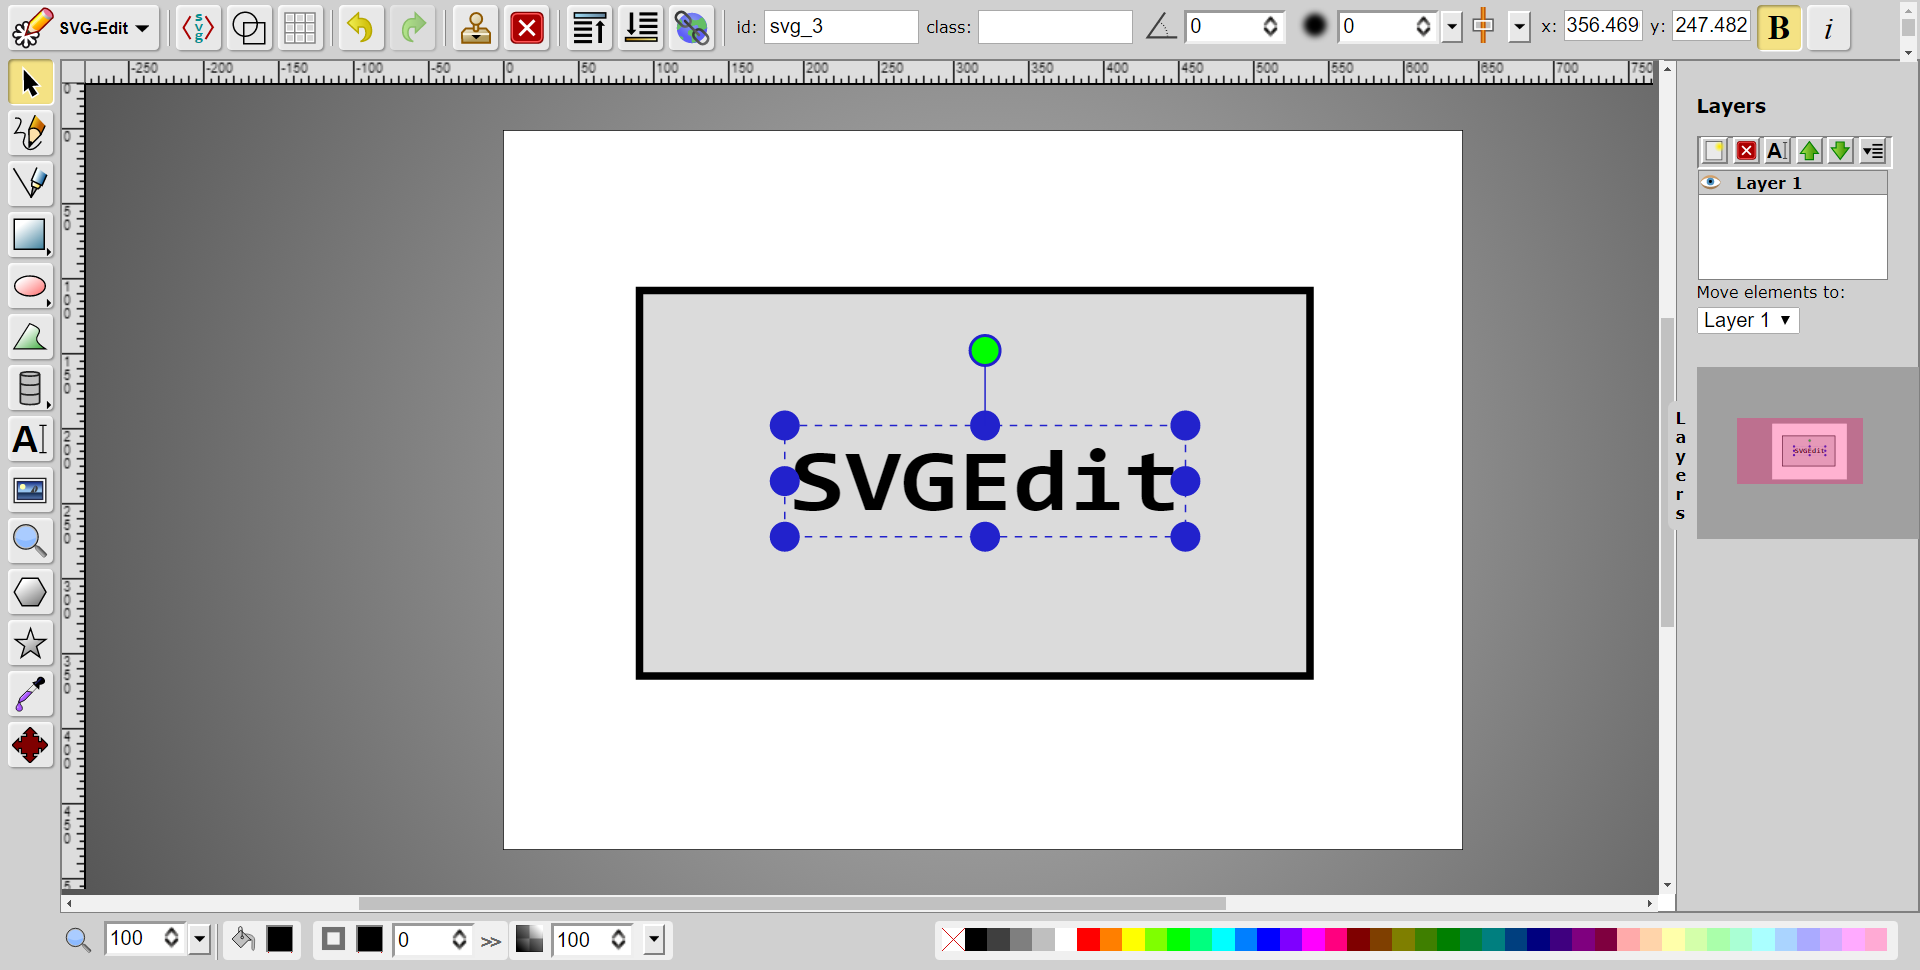
\includegraphics[width=1\textwidth]{images/svg-edit}}
	\caption[Editor SVG-edit]{Prostredie editora SVG-edit}
	\label{obr:SVGedit}
\end{figure}
\FloatBarrier


\section{Figma}

Figma je profesionálny grafický editor s možnosťou kolaboratívnej práce viacerých používateľov. Je určený predovšetkým pre ľudí zaoberajúcich sa grafickým návrhom mobilných, webových alebo desktopových aplikácií. Jeho hlavnou výhodou je intuitívne ovládanie, real-time komunikácia medzi spolupracujúcimi používateľmi a bohatá funkcionalita. 

Keďže sa však jedná o samostatný webovú aplikáciu nieje možné ju implementovať do MediaWiki systému.

\begin{figure}[h]
	\centerline{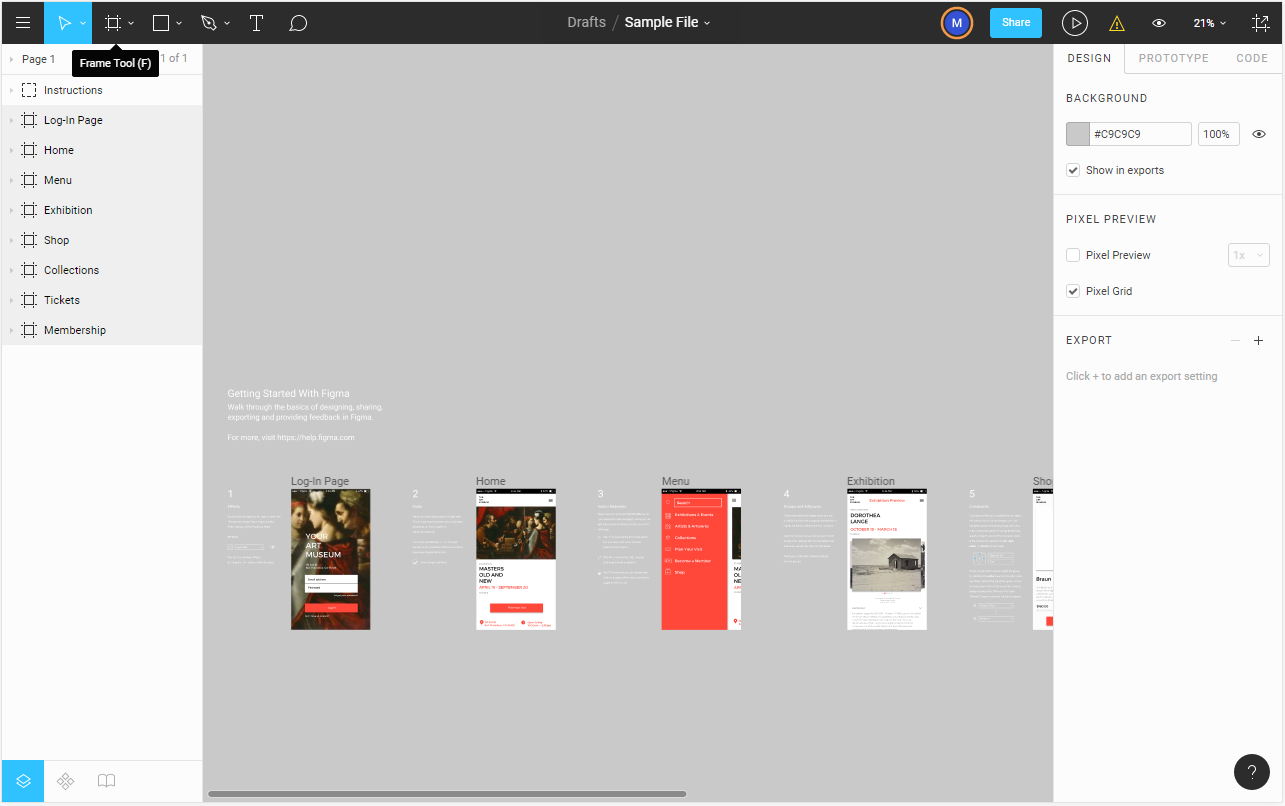
\includegraphics[width=1\textwidth]{images/figma}}
	\caption[Editor Figma]{Prostredie kolaboratívneho editora Figma}
	\label{obr:Figma}
\end{figure}
\FloatBarrier

\section{Draw.IO}
\textit{Draw.IO} je pomerne známy editor, určený na kolaboratívnu tvorbu vektorovej počítačovej grafiky. Primárne je používaný na tvorbu diagramov, 


\begin{figure}[h]
	\centerline{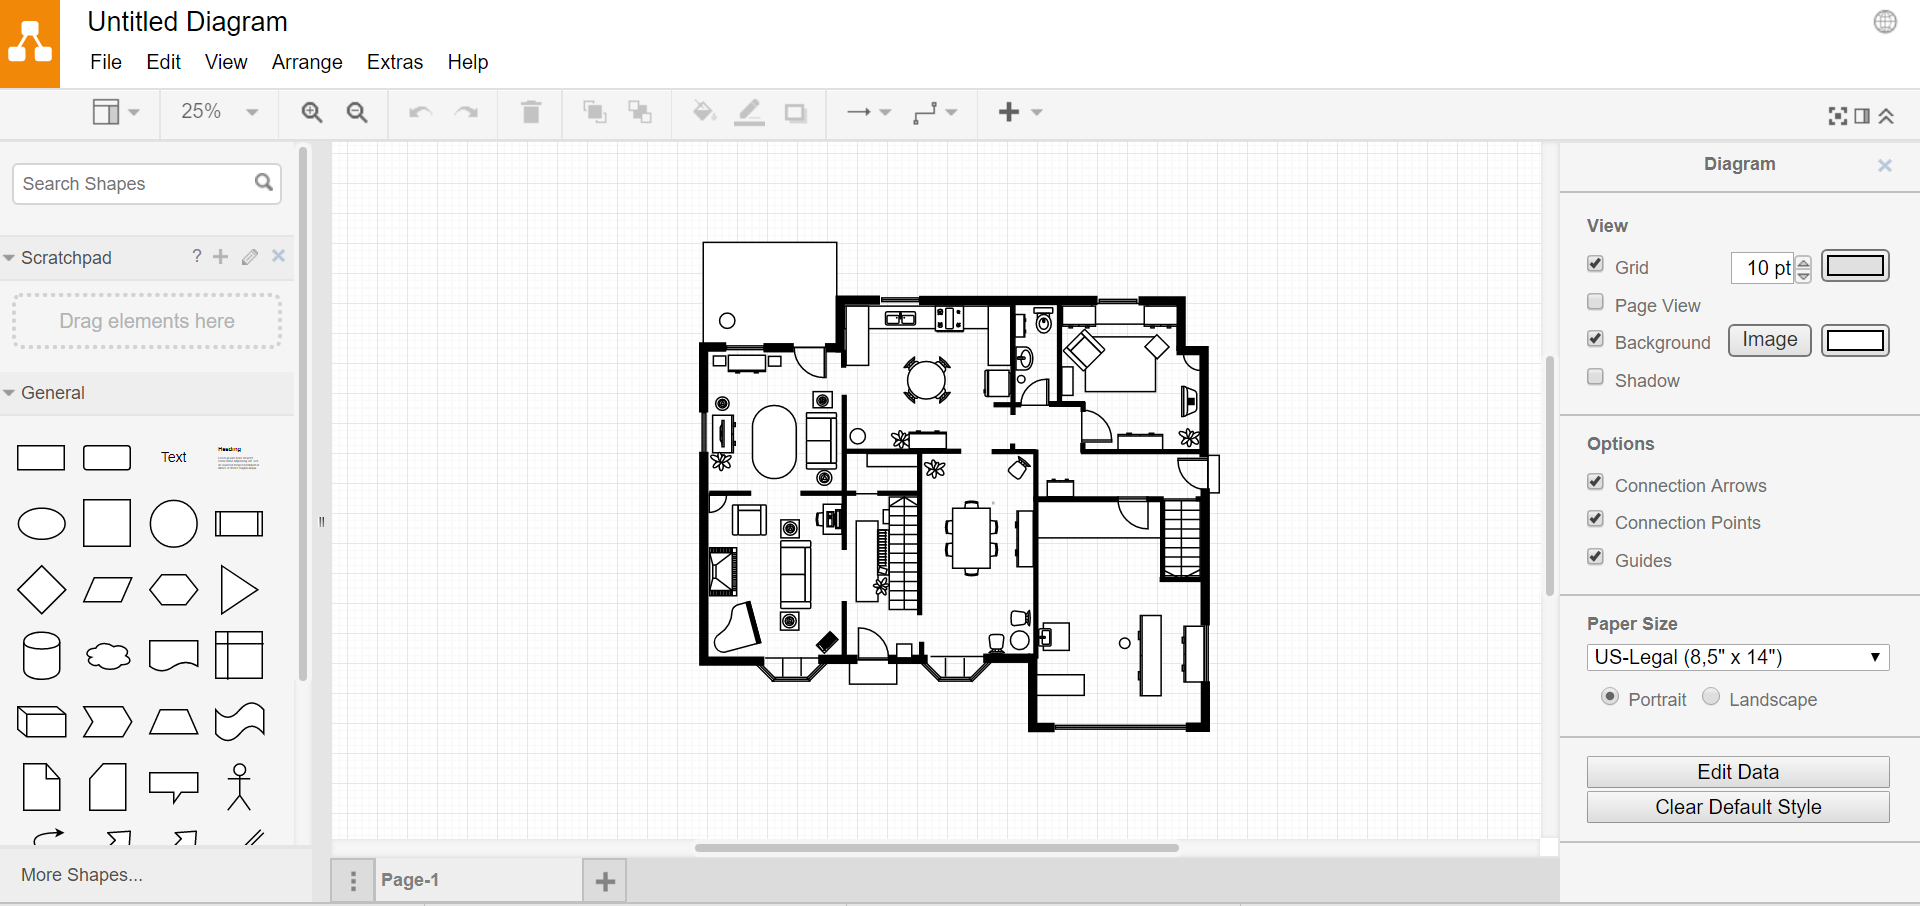
\includegraphics[width=1\textwidth]{images/drawio}}
	\caption[Editor Draw.IO]{Prostredie kolaboratívneho editora Draw.IO}
	\label{obr:DrawIO}
\end{figure}
\FloatBarrier